\documentclass{llncs}
\usepackage{amssymb}
\usepackage{amsmath}
\usepackage{algorithm}
\usepackage{algpseudocode}
\usepackage{graphicx}
\usepackage{epstopdf}
\usepackage[draft,margin]{fixme}

%\usepackage{float}

%\newtheorem{dfn}{Definition}{}
%\newtheorem{thm}[dfn]{Theorem}{}
%\newtheorem{cor}[dfn]{Corollary}{}
%\newtheorem{prb}{Problem}{}
%\newtheorem{lem}[dfn]{Lemma}{}
%\newtheorem{algx}[dfn]{Algorithm}{}

\newcommand{\bigo}{\mathcal{O}}
\renewcommand{\mod}{\text{ mod }}
\newcommand{\E}{\mbox{\rm \bf{E}}}
\renewcommand{\Pr}{\mbox{\rm \bf{Pr}}}
\newcommand{\Var}{\mbox{\rm \bf{Var}}}
\newcommand{\Xac}{X_{(a,c)}}
\newcommand{\mcA}{\mathcal{A}}
\newcommand{\mcB}{\mathcal{B}}
\newcommand{\mcC}{\mathcal{C}}

\newcommand{\ordo}[1]{{\cal O}\left(#1\right)}
\newcommand{\ordop}[1]{{\cal O}^*\left(#1\right)}
\newcommand{\calG}{\mathcal{G}}
\newcommand{\calH}{\mathcal{H}}
\newcommand{\calE}{\mathcal{E}}
\newcommand{\calX}{\mathcal{X}}
\newcommand{\calS}{\mathcal{S}}
\newcommand{\calT}{\mathcal{T}}
%\newcommand{\qed}{\hfill \ensuremath{\Box}}

\newtheorem{defx}{Definition}
\newtheorem{lemmx}{Lemma}
\newtheorem{thmx}{Theorem}
\newtheorem{algx}{Algorithm{\\}}
\newtheorem{procx}{Procedure}

\newenvironment{procedure}{\begin{procx}\em \footnotesize}{\end{procx}}

% These are used indirectly by the following group of new environments


%%\newcommand{\e}{\epsilon}
\begin{document}


\title{Does past stock performance matter in investing?}
\date{}
\author{Konstantin Kutzkow and Kevin Tierney}
\institute{}
\maketitle
\begin{abstract}
In our project we investigate the impact of past stock data on future price movement. More precisely, we consider two different approaches for predicting the future stock behavior: supervised learning based on feature vectors built from technical analysis indicators, and  sequence mining for discovering frequent patterns of stock price movements for a given stock. %{\em Optional: We also investigate the relationship between price movements for different stocks and use this to prediction of stock prices.}
\end{abstract}
\section*{Data}
We gathered publicly available data from Yahoo! Finance for different stocks in two sectors: Basic materials and Technology. For all stocks the complete price history is available. The Basic materials sector consists of companies involved with the discovery, development and processing of raw materials such as metals, chemical producers and forestry products. The Technology sector contains stock data for companies in areas like software development, electronics manufacturing, and other businesses related to information technology.

The Basic materials sector contains data for stocks positively correlated with a strong economy, e.g. the stocks of companies producing steal are dependent on the automotive industry, as well as stocks negatively correlated with the economic growth, e.g. the demands for gold rise during a bad economy cycle.

On the other hand, the technology sector has experienced a boom in the last 20 years and we would like to investigate whether the stock prices for different stocks behave in a similar way. 

For our project we used the price history for 42 stocks in the technology sector and 31 stocks in the basic materials sector. 
\section*{Data preprocessing}
For each stock we are provided with a csv file consisting of the following features for the stock for each trading day: opening price, closing price, highest and lowest price and the volume of traded stocks for the day. We directly use the numerical values in order to compute technical analysis indicators and to label days, respectively longer time periods, in a way describing in an informative manner the behavior of the stock for the considered time interval. 

Note that since our data contains no missing or inconsistent values no data cleaning is necessary. Further, we chose to work with the exact numerical values for each stocks, thus no data discretization or clustering was applied.

In the next sections we explain in details which transformations were used in order to extract meaningful information from the exact numerical values of the stock prices.
\section*{Supervised learning}
We incorporate several technical indicators about past stock behavior into feature vectors. We label the data as follows...
 
\section*{Frequent pattern mining}
\subsection*{Motivation}
The idea is to find frequently occurring patterns of price movements. Unlike in the previous section we do not acquire any information from stock technicals. The intuition is to try to detect price movement dependencies in a more direct way by simply considering the past stock performance. The intuition is that sometimes technicals might give too much information which dilutes the picture we want to analyze, namely how does the price curve look.

Consider for example the graph of the curve for the stock price movement of Adobe for the period from 1994-07-13 to 1995-04-27. We see there are certain reoccurring patterns, for example a sharp fall is followed by a sharp rise of the price in three different situations: (label somehow the picture...) 

\begin{figure}[htb!]
\caption{Price movement for Adobe stocks}
\centering%
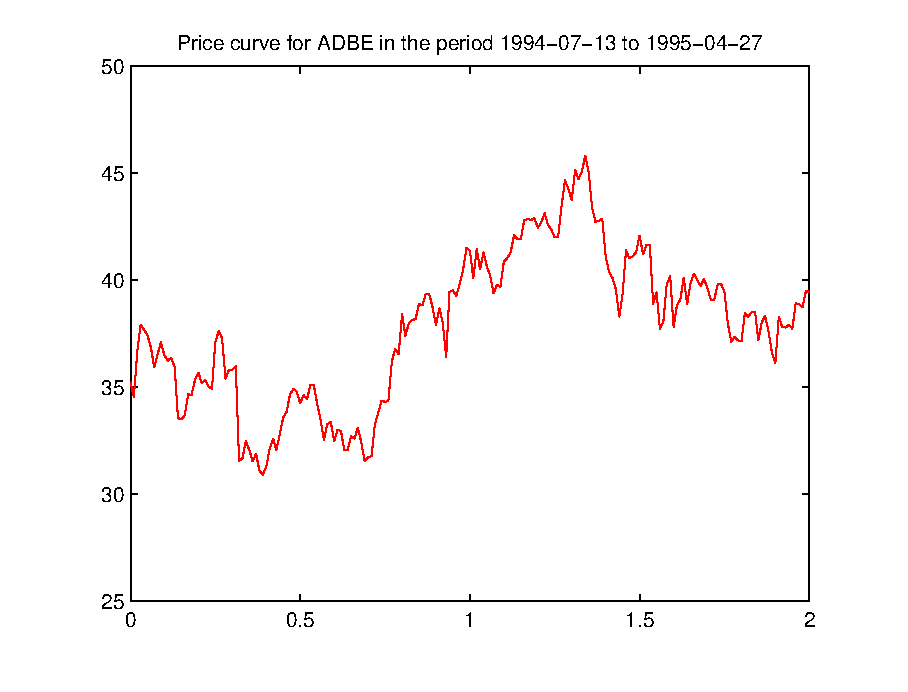
\includegraphics[scale=0.7]{ADBE.eps}
\end{figure}

\subsection*{General setting}
We consider the price movement of a given stock over a certain time period. We divide the period in small subintervals of at least one day which we consider data points in a sequence.  
We label the data points such that the label indicates the stock price movement. We use three distinct labels $F, H$ and $R$ indicating whether a given price will decrease its value over a given period ($F$), will retain approximately the same value ($H$), or will increase its price ($R$). They are obtained depending on the opening and closing price for the period. 
\subsection*{A modified Apriori approach}
Let us formally define our problem.

We are given a sequence $\mathbb{S}$ of symbols $s \in \mathcal{A}$ over some alphabet $\mathbb{A}$. Let the support of a subsequence $S \subseteq \mathbb{S}$ be $\mbox{sup}(S) = \frac{\#S}{|\mathbb{S}| - |S|}$ where $\#S$ is the number of occurrences of the subsequence $S$ in $\mathbb{S}$ and $|\mathbb{S}|$ and $|S|$ are the lengths of $\mathbb{S}$ and $S$, respectively. That is, the support of a given sequence $S$ is the number of its occurrences divided by the number of all subsequences in $\mathbb{S}$ of length $|S|$.  For a given support threshold $\sigma$ and a confidence threshold $\tau$ we want to find all subsequences $S \subset \mathbb{S}$ such that $\mbox{sup}(S) \geq \sigma$ and $\mbox{conf}(S) \geq \tau$. The confidence $\mbox{conf}(S)$ of a rule derived from $S$ is defined as $\frac{\mbox{sup}(S)}{\mbox{sup}(S\backslash\ell)}$ where $\ell$ is the last symbol in $S$.

Obviously, the above definitions are similar to the itemset and transaction setting in the classic frequent pattern mining context. However, an important difference is that one can build only linearly many subsequences of a given sequence, thus the following algorithm avoids the combinatorial explosion caused by Apriori for lower support thresholds and is thus much more efficient. %(Note that our algorithm is different from the one proposed in \cite{fpstock}.)
\\
\begin{algx} {Frequent sequence mining}
\begin{enumerate}
\item Find frequent symbols, set $k=2$.
\item Join frequent subsequences of length $k-1$ if the last $k-2$ symbols of the first subsequence are identical to the first $k-2$ symbols of the second subsequence
\item build a set of candidates of length $k$ and filter out infrequent subsequences.
\item repeat steps 2--3 until no new frequent subsequences can be obtained.
\end{enumerate}
\end{algx}
\begin{lemmx}
The algorithm correctly identifies all frequent subsequences of a given sequence.
\end{lemmx}
\begin{proof}
For a subsequence $S$ to be frequent the Apriori property that all proper subsequences $S'$ of $S$ are frequent must hold. Thus, assuming we have identified all frequent subsequences of length $k-1$, steps 2 and 3 return a superset of the frequent subsequences of length $k$. Correctness follows by a simple inductive argument. \qed
\end{proof}

{\bf Example:}  Let us consider a simple concrete example: the sequence $\mathcal{S} = abcbca ababca abccba abbabc bcacba$ contains 30 symbols. We are interested in all $k$-subsequences with frequency at least 0.15, i.e. occurring in at least 10\% of all subsequences of length $k$. The 1-subsequences are the symbols themselves and we find that all of them are frequent since they appear more than 4.5 times ($4.5 = 0.15\cdot 30$). Then we build candidate subsequences as $aa, ab, ac, ba, bb, bc, ca, cb, cc$ since they all satisfy the joining condition: the last 0 symbols of the first subsequence agree with the first 0 symbols of the second one. From these symbols we find that the subsequence $aa$ appears only once, $ab$ -- five times, $ac$ -- one time, $ba$ -- 4 times, $bb$ -- one time, $bc$-- 6 times, $ca$ -- three times, $cb$-- three times and $cc$ -- one time. The total number of 2-subsequences is 29, thus threshold is now $0.15 \cdot 29 = 4.35$. Thus, the frequent 2-subsequences are $ab$, $ba$ and $bc$. From these we build the following candidate 3-subsequences: $aba$, from $ab$ and $ba$, $bab$, from $ba$ and $ab$, and $abc$, from $ab$ and $bc$. Note that $ba$ and $bc$ can not be combined since they don't satisfy the joining condition. Now $aba$ appears only once, $bab$ twice, and $abc$ -- four times. Thus, no 3-subsequence is frequent, i.e. occur more than $4.2 = 0.15\cdot 28$ times, and the algorithm terminates.

In the very same way as in Apriori one computes the confidence of each rule.

\subsection*{Results}
\subsubsection*{Labeling}
We experimented with several values for the number of labels. It turns out that the more labels we have the more difficult it becomes to detect any frequent subsequences for a reasonable support threshold. Thus, we choose to present results when only three labels are used.  

As already mentioned, the three different labels $F, H$ and $R$ indicate whether the price will fall, remain relatively the same, or raise in the considered time period $t$, respectively. The labels are obtained in a natural way: given some threshold $\tau$, we compute the value $f:=\frac{c-o}{c}$ where $c$ is the closing price for the considered period $t$, and $o$ is the opening price. Note that we divide by $c$ in order to achieve normalization not depending on the absolute values of the stock price. Then we label $t$ as $H$ if $-\tau \leq f \leq \tau$, as $F$ if $f < -\tau$, and as $R$ otherwise. 

It is in general a difficult problem to choose an optimal threshold $\tau$, since choosing a small value will lead to labeling periods as either $F$ or $R$ even for non-significant changes of the stock price. On the other hand, big values of $\tau$ result in too many periods labeled as $H$ and this makes it difficult to mine rules with consequent different from $H$.  We observed that values of about $0.1$ give a balanced distribution among labels for most stocks for short time periods and allow the mining of reasonable amount of rules. 

We also experimented with labeling different time periods: it seems that for longer periods valuable information for price movements within the period is lost, while for some stocks for short periods like one day it is difficult to capture the effect of, say, more slowly price movement.  

\subsubsection{Choosing the best rule}
In certain situations we might be able to apply more than one rule. For example, the labels for the last three time periods are $HHF$ and we have the rules $HF \rightarrow F$ and $HHF \rightarrow H$. The most natural choice is the rule with the best confidence. However, a rule with a longer antecedent might give us better information since it takes into account more information. We implemented both strategies. It is difficult to say which one performs better, since apparently different stocks behave differently.  

\subsubsection{Average correctness}

After labeling the data for a given stock over a certain time period, say 3 days, we perform frequent sequence mining over the sequence. We use the first $2/3$ of the sequence for frequent pattern mining, and the last $1/3$ for applying our rules and correctness testing of our predictions. For all considered stocks we mined the sequences for the whole price history. 

The following table shows the label distribution and the percentage of correct predictions we obtain for certain stocks from the technology sector for threshold $\tau = 0.012$ and label period $t=2$. A more comprehensive list can be found in the appendix.
\\\\
\begin{tabular}{| l | l | l | l | l |}
\hline
Stock & average F & average R & average H & correct predictions\\
\hline
  AAPL & 0.3490 & 0.2935 & 0.3574 & 0.3888\\
\hline
  ADBE & 0.3476 & 0.2828 & 0.3695 & 0.3805 \\
\hline 
DELL & 0.32164 & 0.3154 & 0.3628 & 0.3823\\
\hline
  HPQ & 0.2973 & 0.3819 & 0.3207 & 0.3333 \\
\hline
MSFT & 0.2839 & 0.4013 & 0.3146 & 0.5702\\
\hline
WFR & 0.3988 & 0.2172 & 0.3839 & 0.4628\\
\hline
\end{tabular}
\\\\
A similar table for the basic materials sector with $\tau = 0.009$ and $t=2$:
\\\\
\begin{tabular}{| l | l | l | l | l |}
\hline
Stock & average F & average R & average H & \% correct predictions\\
\hline
ADM & 0.38 & 0.248 & 0.3716 & 0.4006\\
\hline
AVP & 0.3516 & 0.2838 & 0.3644 & 0.3841\\
\hline
MKC & 0.2774 & 0.4095 & 0.3129 & 0.3435\\
\hline
NWL & 0.3618 & 0.2701 & 0.3680 & 0.4640\\
\hline
RAI & 0.2638 & 0.4146 & 0.3214 & 0.3846\\
\hline
TAP & 0.3192 & 0.3412 & 0.3394 & 0.3946\\
\hline

\end{tabular}
\\\\
As one can see, different stocks behave differently and for example Microsoft turns out to be much more predictive than Hewlett-Packard. Nevertheless, for all stocks the percentage of correct predictions is significantly better than guessing at random based solely on the labels distribution. 
We observe that the higher threshold $\tau$ we choose, i.e. we are more conservative in labeling a price movement as $F$ or $R$, the better predictions we get. See Figure 2. This has two explanations: First, most rules should have consequent $H$, thus simply predicting $H$ for each next day should also give a good estimate. On the other hand, as one clearly sees from the graphic the percentage of correct predictions is growing faster than the percentage of $H$ labels. The intuitive explanation is that the price movement becomes less sensitive to small oscillations.
%We obtain the following results for chosen stocks:
\begin{figure}[htb!]
\caption{Correctness}
\centering%
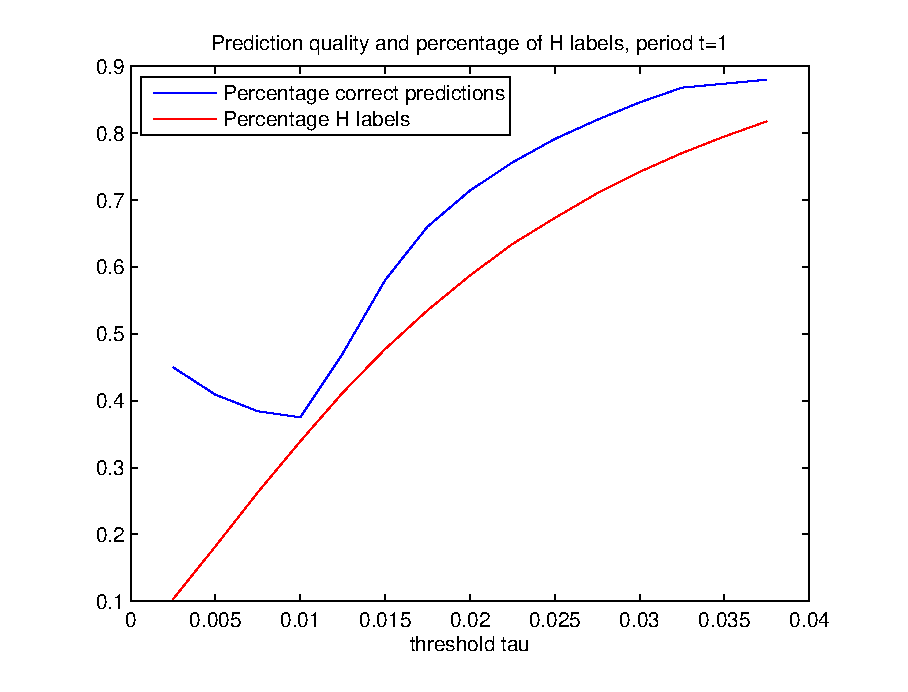
\includegraphics[scale=0.7]{corr.eps}
\end{figure}
\subsection*{Can we become rich?}
One obvious question that arises is how to use the discovered knowledge to make some profit. First of all, we would like to distinguish between {\em knowledge discovery} and {\em use of the discovered knowledge}. An experienced investor can use the mined rules in a much cleverer way and the primary goal of this project is applying data mining techniques for discovering knowledge, not a real world application of the discovered knowledge. Nevertheless, out of curiosity, we implemented the following simple strategy: If our rule for the next day predicts $R$ we buy 10 stocks in the morning and sell them in the evening, thus our revenue is $10\cdot (close\_price - open\_price)$. Note that since we are buying and selling stocks in the same day, the effect inflation has on the stock price movement is minimized.  We obtained following revenues for different stocks:
\\\\
\begin{tabular}{| l | l | l || l | l | l |}
\hline
Stock & Prediction & Revenue & Stock & Prediction & Revenue\\
\hline
AAPL & 0.3765 & 207.3 & ADI & 0.3624 & 23.6\\
\hline
ADSK & 0.2866 & 13.6 &  ALTR & 0.3921 & 0\\
\hline
AMD & 0.3702 & -39.6 & BMC & 0.5142 & 55.19\\
\hline
DELL & 0.4773 & 0.0 & EMC & 0.3916 & -8.1\\
\hline
FFIV & 0.3609 & 157.2 & FLSR & 0.29 & -306.1\\
\hline
NVDA & 0.3315 & 33.5 & MSFT & 0.6155 & 0.0\\
\hline
\end{tabular}
\\\\We wanted to check whether a more conservative labeling strategy would yield better revenue. The Figure 3 table summarizes the average revenue over all 42 stocks in the technology sector. As one can see, despite some fluctuations, the average revenue drops for higher values of $\tau$, i.e. more labels $H$. 
\begin{figure}[htb!]
\caption{Average revenue depending on labeling strategy.}
\centering%
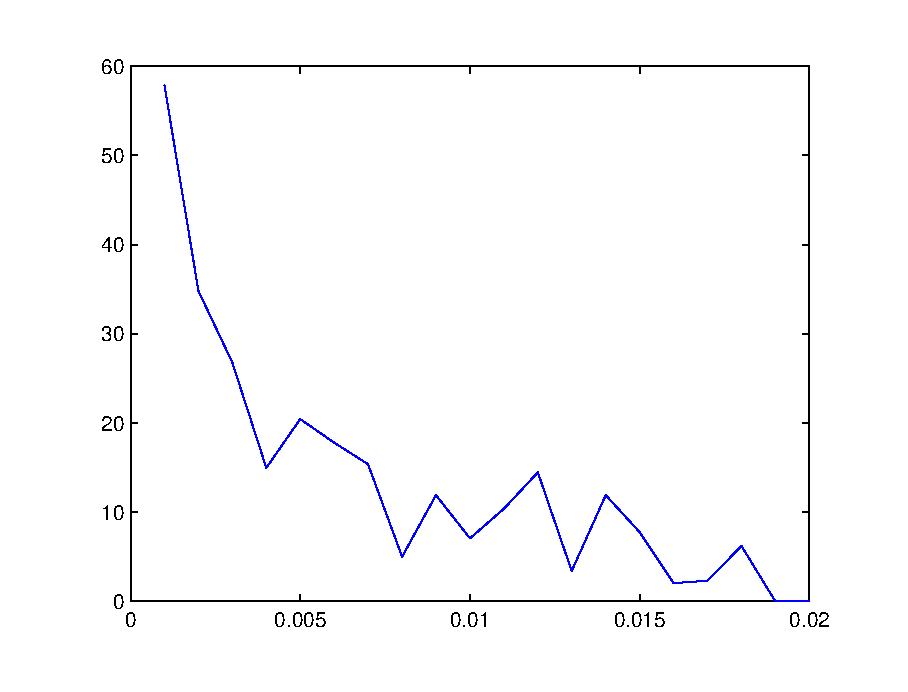
\includegraphics[scale=0.7]{revenue.eps}
\end{figure}

\section*{Conclusions}
Obviously, our algorithms detect some dependencies in the price movement for a given stock and also for the price movement in a whole sector. However, there are considerable differences even among stocks in the same sector.

The frequent pattern mining part of the project clearly shows that certain rules can be mined and for most of the stocks they turn out to be to some degree accurate. However, a much deeper research is required in order to analyze which requirements should a stock satisfy in order to obtain a reliable labeling. Apparently, simply dividing stocks into sectors is not enough and more subtle subdivision needs to be performed. It is in general questionable whether approaches based on ``purely" frequent pattern mining techniques can be successful since they only take into account the price movement. A more promising direction would be to use frequent pattern mining in combination with other techniques in order to support the prediction based on other methods. But such a study is beyond the scope of a course project.  
%\subsection*{Correlation pattern mining}
%It is often the case that the price movement of a certain stock is correlated with the prices of other stocks. For example higher prices for metals will affect negatively the automotive industry but the effect occurs after some time. Another example is...
%
%Inspired by the above we implemented a sequence mining algorithm for detecting correlations between stocks within a given time span. For example is there a correlation between the price movement of stock $A$ in the interval $[p, q]$ and the price of stock $B$ in day $q+t$ for some appropriately chosen $t$. We experimented with different time intervals in order to mine dependencies between the stocks.

%\begin{thebibliography}{1}
%\bibitem{fpstock}
%Jo Ting, Tak-Chung Fu, Fu-Lai Chung: 
%\newblock Mining of Stock Data: Intra- and Inter-Stock Pattern Associative Classification. \newblock {\em DMIN 2006:} 30--36
%\end{thebibliography}

\section*{Appendix}
\begin{verbatim}
AAPL.txt
F : 0.29525483304042177
H : 0.36379613356766255
R : 0.3409490333919156
correctness = 0.3888888888888889
+++++++++++++++++++++++++++++++++++++++
ADBE.txt
F : 0.2827324478178368
H : 0.40037950664136623
R : 0.31688804554079697
correctness = 0.3333333333333333
+++++++++++++++++++++++++++++++++++++++
ADI.txt
F : 0.2972027972027972
H : 0.4195804195804196
R : 0.28321678321678323
correctness = 0.271356783919598
+++++++++++++++++++++++++++++++++++++++
ADSK.txt
F : 0.29891304347826086
H : 0.3351449275362319
R : 0.36594202898550726
correctness = 0.36220472440944884
+++++++++++++++++++++++++++++++++++++++
ALTR.txt
F : 0.31237322515212984
H : 0.36511156186612576
R : 0.3225152129817444
correctness = 0.33557046979865773
+++++++++++++++++++++++++++++++++++++++
AMAT.txt
F : 0.3087719298245614
H : 0.3508771929824561
R : 0.34035087719298246
correctness = 0.368
+++++++++++++++++++++++++++++++++++++++
AMD.txt
F : 0.4276206322795341
H : 0.21963394342762063
R : 0.3527454242928453
correctness = 0.3786764705882353
+++++++++++++++++++++++++++++++++++++++
BMC.txt
F : 0.2511111111111111
H : 0.4288888888888889
R : 0.32
correctness = 0.5342465753424658
+++++++++++++++++++++++++++++++++++++++
BRCM.txt
F : 0.3140794223826715
H : 0.34296028880866425
R : 0.34296028880866425
correctness = 0.3333333333333333
+++++++++++++++++++++++++++++++++++++++
CPWR.txt
F : 0.2557544757033248
H : 0.4040920716112532
R : 0.340153452685422
correctness = 0.29285714285714287
+++++++++++++++++++++++++++++++++++++++
CTSH.txt
F : 0.2564102564102564
H : 0.38095238095238093
R : 0.3626373626373626
correctness = 0.41333333333333333
+++++++++++++++++++++++++++++++++++++++
CTXS.txt
F : 0.2782874617737003
H : 0.3302752293577982
R : 0.39143730886850153
correctness = 0.2916666666666667
+++++++++++++++++++++++++++++++++++++++
DELL.txt
F : 0.3216494845360825
H : 0.3154639175257732
R : 0.3628865979381443
correctness = 0.38235294117647056
+++++++++++++++++++++++++++++++++++++++
EMC.txt
F : 0.3054393305439331
H : 0.3410041841004184
R : 0.35355648535564854
correctness = 0.34210526315789475
+++++++++++++++++++++++++++++++++++++++
ERTS.txt
F : 0.33555555555555555
H : 0.35333333333333333
R : 0.3111111111111111
correctness = 0.3805309734513274
+++++++++++++++++++++++++++++++++++++++
FFIV.txt
F : 0.2896825396825397
H : 0.28174603174603174
R : 0.42857142857142855
correctness = 0.2777777777777778
+++++++++++++++++++++++++++++++++++++++
FSLR.txt
F : 0.3010752688172043
H : 0.3978494623655914
R : 0.3010752688172043
correctness = 0.2982456140350877
+++++++++++++++++++++++++++++++++++++++
HPQ.txt
F : 0.24383301707779886
H : 0.43833017077798864
R : 0.3178368121442125
correctness = 0.3333333333333333
+++++++++++++++++++++++++++++++++++++++
INTC.txt
F : 0.27547169811320754
H : 0.44528301886792454
R : 0.2792452830188679
correctness = 0.2962962962962963
+++++++++++++++++++++++++++++++++++++++
INTU.txt
F : 0.21558441558441557
H : 0.44935064935064933
R : 0.33506493506493507
correctness = 0.3014705882352941
+++++++++++++++++++++++++++++++++++++++
KLAC.txt
F : 0.3422222222222222
H : 0.31333333333333335
R : 0.34444444444444444
correctness = 0.2641509433962264
+++++++++++++++++++++++++++++++++++++++
LLTC.txt
F : 0.29777777777777775
H : 0.3977777777777778
R : 0.30444444444444446
correctness = 0.3488372093023256
+++++++++++++++++++++++++++++++++++++++
LSI.txt
F : 0.3634361233480176
H : 0.2687224669603524
R : 0.36784140969163
correctness = 0.36
+++++++++++++++++++++++++++++++++++++++
MHCP.txt
F : 0.2927461139896373
H : 0.40932642487046633
R : 0.2979274611398964
correctness = 1.0
+++++++++++++++++++++++++++++++++++++++
MSFT.txt
F : 0.2718808193668529
H : 0.4692737430167598
R : 0.25884543761638734
correctness = 0.5702479338842975
+++++++++++++++++++++++++++++++++++++++
MU.txt
F : 0.4157782515991471
H : 0.2260127931769723
R : 0.3582089552238806
correctness = 0.38181818181818183
+++++++++++++++++++++++++++++++++++++++
NOVL.txt
F : 0.29545454545454547
H : 0.4256198347107438
R : 0.27892561983471076
correctness = 0.3305785123966942
+++++++++++++++++++++++++++++++++++++++
NSM.txt
F : 0.34609250398724084
H : 0.34290271132376393
R : 0.31100478468899523
correctness = 0.3473053892215569
+++++++++++++++++++++++++++++++++++++++
NTAP.txt
F : 0.2978723404255319
H : 0.2765957446808511
R : 0.425531914893617
correctness = 0.3644067796610169
+++++++++++++++++++++++++++++++++++++++
NVDA.txt
F : 0.32950191570881227
H : 0.2796934865900383
R : 0.39080459770114945
correctness = 0.33884297520661155
+++++++++++++++++++++++++++++++++++++++
NVLS.txt
F : 0.35777777777777775
H : 0.27555555555555555
R : 0.36666666666666664
correctness = 0.4090909090909091
+++++++++++++++++++++++++++++++++++++++
ORCL.txt
F : 0.27111111111111114
H : 0.4177777777777778
R : 0.3111111111111111
correctness = 0.460431654676259
+++++++++++++++++++++++++++++++++++++++
RHT.txt
F : 0.27309236947791166
H : 0.3855421686746988
R : 0.3413654618473896
correctness = 0.2682926829268293
+++++++++++++++++++++++++++++++++++++++
SAI.txt
F : 0.16842105263157894
H : 0.6736842105263158
R : 0.15789473684210525
correctness = 0.6666666666666666
+++++++++++++++++++++++++++++++++++++++
SNDK.txt
F : 0.3556231003039514
H : 0.22188449848024316
R : 0.42249240121580545
correctness = 0.3935483870967742
+++++++++++++++++++++++++++++++++++++++
SYMC.txt
F : 0.3
H : 0.4177777777777778
R : 0.2822222222222222
correctness = 0.2894736842105263
+++++++++++++++++++++++++++++++++++++++
TER.txt
F : 0.3688888888888889
H : 0.26222222222222225
R : 0.3688888888888889
correctness = 0.3680555555555556
+++++++++++++++++++++++++++++++++++++++
TXN.txt
F : 0.3
H : 0.37555555555555553
R : 0.3244444444444444
correctness = 0.24675324675324675
+++++++++++++++++++++++++++++++++++++++
VRSN.txt
F : 0.23843416370106763
H : 0.4199288256227758
R : 0.3416370106761566
correctness = 0.273972602739726
+++++++++++++++++++++++++++++++++++++++
WDC.txt
F : 0.36
H : 0.24888888888888888
R : 0.39111111111111113
correctness = 0.46875
+++++++++++++++++++++++++++++++++++++++
WFR.txt
F : 0.39880952380952384
H : 0.21726190476190477
R : 0.38392857142857145
correctness = 0.4628099173553719
+++++++++++++++++++++++++++++++++++++++
XLNX.txt
F : 0.28314606741573034
H : 0.36404494382022473
R : 0.35280898876404493
correctness = 0.31958762886597936
\end{verbatim}

\end{document}
